
  \chapter{Optimal Service Placement in a Virtualized Environment}  
  \label{ch:optimization-virtualized} 
  In chapter \ref{ch:optimization}  we analyzed the end-to-end  Management of service center, where number of service replicas and placement of these replicas was obtained by solving a single optimization problem.  
 Using virtualization, it is possible to offer infrastructure in terms of small chunks, namely virtual machines. As a IaaS user, we use the virtual machines as unit's of hardware with isolated and consistent performance attributes. The infrastructure as a service (IaaS) layer   solves the placement problem for virtual machines on available hosts in a way that it satisfies hardware layer goals regarding consolidation or homogeneous utilization. Thus, one can use IaaS and focus on provisioning of services using virtual machines.  

 \section{The Formulation}
Lets assume virtual machines are grouped into a set of $Cl$ clusters based on services they host. Each cluster is homogeneous; % in the sense that every virtual machine within a cluster meaning that it hosts the same set of services that has the same virtual machine specification. Each service can span multiple clusters. Let us assume  $m_{cl}$ represents the number of machines in cluster $cl$.  
   Recalling from chapter \ref{ch:optimization}, the physical workload imposed on resource $k'$ of host $h$ from customers of class $c$ accessing service $s$ is calculated by the expression: $X_c (V_{c,s} \theta_{s,h}) D_{s,k'}$.   Further, let's assume within each cluster $cl$ the resource usages are distributed equally between all the hosts  ($\theta_{s,h}$ are equal  for each cluster). With these assumptions, each cluster can be modeled as a shared queue multi-server, which can be approximated, by a queuing centre and a delay centre. The new service demands of the cluster are then derived as $d_{c,s}\theta_{s,cl}= V_{c,s} D_s \theta_{s,cl}$. 
   
   To further simplify the problem, let us assume all the classes in the system are aggregated into one class. Then the high level objectives can be described in terms of aggregated throughput $X$ and response time $R$.   % As a result demand of each service on that type of virtual machine is only indexed by the service, $D_s$.  In addition, in this case, on each virtual machine a single replica of a service is deployed. 
  Then targeting only cluster $cl$, demand of each cluster can be derived as sum of the demands of services deployed on the cluster considering the the multi-cluster services 
  $d_{cl}=\sum_s d_{c,s}\theta_{s,cl}$.    % $d_{cl}=\sum_s d_{s,cl}$. 

%  instead of  service demands in terms of class–service–resource type
%   in this chapter we index demand in terms of class–cluster–resource type. 
% 
%  instead of $D_s$ which includes $d_{c,s}=V_{c,s} D_s$  and gets  distributed  
%  between hosts as $d_{c,s,h,k'}=X_c (V_{c,s} \theta_{s,h}) D_{s,k'}$, 
%  
%   where cl is considered a multi-server shared queue resource. 
  

  \section{Sub-Optimal Autoscaling through Utilization Control}   % Stationary Policy  
 %  \subsection{suboptimal solution  heuristic PID utilization control}  
  \label{sec:non-optimal-autoscaling}   
 
   Utilization control as a way to regulate high-level performance metrics such as throughput has been investigated in different contexts than service centre autoscaling \cite{kalyvianaki_self-adaptive_2009}.  In this subsection, we propose solving the autoscaling problem in service centre using the simplistic utilization control.
    The intuition behind this approach is that if increasing multiplicity of a cluster improves the overall throughput, then the utilization experienced by every server in the cluster after autoscaling will not drop as much. This is because increase in the multiplicity is compensated with the extra throughput to be handled. If the autoscaling action has no effect on throughput, the load each individual server in the cluster experiences after scale-up is going to decrease proportional to the increase in the number of added resources. 
       
%   note that the relationship between the utilization and the multiplicity of a resource described as follows:  
%       (i) When a resource is a bottleneck, adding to its multiplicity will result in improving the overall throughput, but utilization of the resource will not drop  while it is the bottleneck. 
%      (ii)  when a resource just exists the bottleneck status, its utilization will drop with addition of its multiplicity. This behaviour follows the formula $U=XD_{\text{queuing}}+XD_{\text{delay}}$. increasing the multiplicity of this resource  does not increase system throughput but lowers the demand   of the  approximated queuing centre and thus utilization of multi-server.     
%      (iii)   After the queue length on the approximated queuing centre goes towards 0, 
%      the utilization of the multi-server goes towards the delay centre's utilization, 
%      $U=XD_{\text{queuing}}+XD_{\text{delay}}$.  
  
  % if a service is a bottleneck then its service rate is low but utilization is low means its a  software bottleneck.
 

%\section{Non-Optimal  Autoscaling of Aggregated Class Workloads}   % Stationary Policy  
%\label{sec:non-optimal-autoscaling}
%
% \textbf{The objectives} of the  lower control  layer are as follows: 
% 
% (1)  \textbf{regulating the  average utilization of  resources} around certain value such as 60\%.  
%   Regulating a  utilization of  a single resource around such value guarantees that the resource is not a bottleneck 
%    for services deployed  on it. In this case the objective function will contain a term denoting a norm of deviation from the target  utilization for  hardware resources  of each host: $\text{minimize} \sum_{t'=1}^{T'} \sum_h (U_{h,t} - 0.6 \capp_h)$). The other way to model the objective is to aggregate utilization of all the hosts into a single distribution and encode the objective in terms of mean and variance of this distribution  (i.e. the distribution of the probability of the machine having certain resource utilization (i.e. $P(\frac{U_h}{\Omega}=U_0)$) obtained from  the current  utilization  level  of hosts (i.e. $\frac{N(\frac{U_h}{\Omega}=U_0)}{H}$ ).  The variance of this distribution   represents the homogeneity of the infrastructure utilization.  Since a target is having a homogeneous cluster or cloud in terms of resources utilization, the target should be minimizing this variance.  Note that there is a trade-off between minimizing the variance of the resource utilizations and the amount of trashing done through change of service books. Also, note that the variance in black box case depends on the performance of the placement algorithm.
   
%  (2) Range Regulation: The controller can also try to regulate the resource utilizations in the range of values rather than around a single point target  (for example between 50\% and 70\%).  In this case the objective function will contain a term that penalizes the excess of the utilization over the upper bound and its shortage below the lower bound: $  \text{minimize} \sum_h \mathtt{pos}(U_h-0.7) + \mathtt{pos}(0.5-U_h) $. In case of the distribution, this objective is the present by putting certain percentile (such as 51\%) of the distribution into the interval 
%  The dynamics of and system and out the autoscaling part are as follows. 

 % one of the current techniques used in industry to manage overall performance  of applications is autoscaling single services based on  some stationary policy.  Although widely used, formalization of this type of policy and its effect on the system performance is not investigated thoroughly. 
 
 % In this subsection to provide the formalization of this type of policy, which can be used as a baseline to be compared to other suggested approaches.
  
    In such system, the end-to-end throughput goal is satisfied if no service is a bottleneck.  Assuming that the multiplicity of software services are high enough not to cause a software bottleneck, the necessary and sufficient condition to satisfy end-to-end throughput goals is that the underlying hardware resources supporting the service are not saturated. By lowering the utilization enough (i.e. 60\%) it is guaranteed that hardware throughput at least equal to the SLA throughput.   
    
    Note that for each service a different type of resource might be the bottleneck for example for database service usually the memory or disk, for a load balancer service the network, and for the application logic services the CPU is a bottleneck. 
     For the cluster that hosts multiple services, finding the bottleneck resource before the deployment is not feasible. Thus at runtime, one has to set the controller targets around the bottleneck resource. In case of multiple bottleneck resources controller should maintain multiple targets (we do not cover this case here.).  
   
         We propose a simple way for controlling the utilization of the cluster using a PID like controller system. Dynamics of such controller system are as follows: 
         \begin{align} 
              x=f(x,\Delta U) \\ 
              y=g(x)
           \end{align}    
  here deviation of system outputs (resource utilizations)  from desired outputs $\Delta U=U^{\text{target}}-U$  is the input to the controller system, and $x$ is the state of the controller.  Note that the output of the controller in each time step depends on past outputs of the system as well as the current one.  
  
   Let's assume $U_{cl,h,k',t}$  represents the utilization of resource type $k$ of host $h$  of cluster $cl$ at time $t$. Then the extent to which a utilization has been breaching a specified threshold is denoted by
    \begin{align}  
      \Delta U_{cl,h,k',t}=U^\text{target}_{cl,k'}-U_{cl,h,k',t}
    \end{align} 
  Lets assume we define a smoothing state 
  \begin{align}  
   \Delta U^\text{smoothing}_{cl,h,k',t} = \alpha_{cl,k'} \Delta U^\text{smoothing}_{cl,h,k',t}+(1-\alpha_{cl,k'})\Delta U_{cl,h,k',t}   
   \end{align} 

   were $\alpha\in[0,1]$  that accumulates the history of utilization breachings of the past.
 The idea is that the autoscaling action for cluster $cl$ at time $t$ is derived by aggregating the tensor $\Delta U^\text{smoothing}_{cl,h,k',t}$ over resource types $k'$  and hosts $h$. Here we aggregate over the resource types of each host by summing the smoothing state:   
\[
\xi_{cl,h,t}=\sum_{k'} \Delta U^\text{smoothing}_{cl,h,k',t} 
\]   
 and aggregate over the hosts  by taking  majority vote: %50 percentile
\[
  \kappa_{cl,t} = \left\{    
  \begin{array}{l l}
    \text{acquire} & \quad \text{if $\left(\sum_{j=1..N} \xi_{cl,h,t}\right)/N > \mathtt{d}$}\\
    \text{release} & \quad \text{if $\left(\sum_{j=1..N} \xi_{cl,h,t}\right)/N < \mathtt{d}$}\\
    \text{none} & \quad \text{otherwise} 
  \end{array} \right. 
\]

Although this controller can be used to constrain the utilization the cluster in an operating region, it has two problems:  
 (i) Controller does not take into account the cost of resources. The resource cost is an implicit side effect of the configuration of the controller. Section ... introduces our new approach to autoscaling that considers the cost.  
 
  (ii) There is no automatic way to find the proper number of alerts, and the associated values for \texttt{a},\texttt{e},\texttt{d} based on the properties of the controller.  However informally we can summarize the effect of these parameters. 
    
   \subsection{Informal Description of Controller Configuration Effects}
We consider the autoscaler described earlier as a transfer function, which takes the output of a service cluster and maps it to actions governing size of the cluster over time.    
Next, we qualitatively categorized the effect of each configuration parameter on this transfer function.

In our experiments all the alerts in all targets were identical and based on the template introduced in Table \ref{tab:alerts-spec-example} (e.g., two alerts where defined, one for scale-up action is case of over-utilization and one for scale-down in case of under-utilization).
Over-utilization is considered when CPU idle time is less than the lower bound \textit{cpu-idle-lb} and underutilization is defined as when CPU idle time is more than the upper bound \textit{cpu-idle-ub}.
The interval $[\text{\textit{cpu-idle-lb}},\text{\textit{cpu-idle-ub}}]$ formed by these two bounds, together with {\it decision threshold}, {\it refractory period}, {\it decision durations}, {\it resize numbers}, and $[\text{{\it min\_instances}},\text{{\it max\_instances}}]$ interval form a simpler configuration space that we investigate in this work. 
We summarize the effect of different autoscaler configurations on the scaling behaviour as follows:

%\begin{description}
\textbf{Operating interval} formed by $[\text{\textit{cpu-idle-ub}},\text{\textit{cpu-idle-ub}}]$ is the main tool in configuring the long term size of the cluster. 
It basically forces the autoscaler to act until the cluster reaches the desired average operating interval (here in terms of CPU idle time, e.g. $[20\%,30\%]$ idle).

If the desired operating interval is located at high CPU idle values (e.g. $[40\%,50\%]$), there will be a lot of instances launched.
Autoscaling will eventually stop due to the increase in the number of idle instances, resulting in less alerts being signaled (as the triggering threshold is no longer reached). 
Notice that the autoscaling action is only performed if the intensity of the workload can get cluster nodes to the desired operating point. Thus, if 
the operating point is configured when nodes are fully utilized (e.g. $[0\%,10\%]$ CPU idle time), the cluster might become unresponsive for low intensity workloads.

If this interval is configured to be narrow and it is placed in an operating area reachable by the workload, it will make the autoscaler sensitive to changes. Such an autoscaler would do some thrashing just to keep the operating point at this narrow interval. If the interval is wide, the cluster will be less responsive, and the cluster utilization will have more space for variations. 

\textbf{Decision duration} contributes to the responsiveness of the cluster. A shorter decision duration for each node results in a quicker response and, thus, it is better at detecting highly variable workloads (e.g. a workload that changes direction every 15 minutes). 
 In case of steady or monotonically increasing/decreasing workloads, the cluster is going to stabilize on a specific size no matter what decision duration is. 

\textbf{Resize numbers} represents the amount of servers to add or remove should a decision threshold (i.e., quorum) be reached  (e.g., 51\%). 
This has a short-term effect on the size of the cluster by making it grow or shrink faster. This might be useful for heavily increasing or decreasing workloads. However, in a long run for a lightly changing workload this might only have effect on smoothness of cluster size over time. 

\textbf{Decision threshold} is global parameter closely related to decision duration, which can affect the responsiveness of the cluster specially in a heterogeneous clusters.
In a heterogeneous cluster, nodes with less processing power might reach the saturation level faster. In this case, a lower decision threshold might result in a better autoscaling decision. The same applied to cluster composed of two different types of nodes (e.g. front-end and application server) where the load on one type of node is higher than the other (e.g. a web application with lots of demand on static resources would result into more utilization at the front-end). 

\textbf{Instance bounds} formed by $[\text{{\it min\_instances}},\text{{\it max\_instances}}]$ acts as constraint on the size of the cluster. 

\textbf{Refractory period} is the interval of time which follows an autoscaling action during which no autoscaling actions may occur.  
% can determine how well the cluster can resize for a changing workload. 
With small refractory periods, the cluster makes resizing decisions more frequently resulting in behavior that is more responsive. 
% \end{description}

\section{Optimal Autoscaling}   
The problem with the utilization controller discussed in section \ref{sec:non-optimal-autoscaling} is that it does not take into account the cost of control,  which is the number of virtual machines used to regulate the utilization. 

 In order to construct an optimal controller we use a queuing model of the system and figure out exactly the amount of needed processing power to accommodate the workload. 
 The system is divided into a set of clusters, where each cluster is homogeneous both in terms of the services it supports and the hardware it has (i.e. the demand of the service on the cluster).  
 The superscript $cl$ is used to represent the a cluster,  
 $d_{c,cl}$ represents the demand of class $c$ on the cluster $cl$.   
 $m_{cl,t}$ denotes the  multiplicity of the cluster $cl$ at time $t$ and 
 $u^\text{m}_{cl,t}$ is the autoscaling action at time $t$ and in the simplest case 
the change in multiplicity of the cluster. 
 
  %  We also overload $m_{{cl},t}$  to denote the multiplicity of internal resources within one instance rather than multiple instances.  We use this overloading when we want to model the vertical scale.
 
%  find the relationship in the form: 
%  \begin{align} 
%    x=f(x,u^\text{m}) \\
%    u=g(x) 
%  \end{align}
% $u^\text{m}$ is the changes in multiplicity of the cluster,  $u$ denotes the average utilization of the cluster, and $x$ represents the state variables necessary
%  to compose the state-space form.    
   
 The problem is finding optimal sequence $u^\text{m}_{cl,t}$ for each $cl$ and $t$. 
  In modeling, we take server multiplicity of each cluster $cl$ over time $m_{cl,t}$ as a state variable. The multiplicity of servers for each cluster is assumed a real value rather than an integer. After finding an optimal real value multiplicity for servers we round it up to obtain a sub-optimal but feasible integer valued answer.
 
  In simplest case the state equation is a simple integration over the changes made on the size of each cluster:
   \begin{align}
    m_{cl,t+1} = m_{cl,t} + u^\text{m}_{cl,t} \label{eq:reservation-dynamics}
  \end{align}

the cost of adding a virtual machine  to a cluster $cl$  depends on the type of virtual machine used in the cluster and the time-step: 
 \begin{align}
   J^\text{cost}_t=\sum_{cl} p_{cl,t} m_{cl,t}  & \qquad \text{for each $cl$ and $t$  }
 \end{align}
 Note that cost is indexed by  timestamp because in a public cloud the prices instance types are subject to change.  
 
   In addition, for monolithic services that are deployed on one host, autoscaling is done by upgrading the instance type to one with more resources (also called vertical autoscaling). In this case, we overload $m_{{cl},t}$  to denote the multiplicity of internal resources within one instance rather than multiple instances. A linear cost function can be obtained by performing a regression of the current prices versus resource multiplicity for different types of instances. After the optimal multiplicity is found by solving the optimization, it is mapped (extrapolated) to the closest instance type with a higher multiplicity.
 
  In order to avoid trashing during autoscaling we associated a cost to an autoscaling action (i.e. changing the number instances in a cluster or upgrading a single instance): 
   \begin{align}
   J^\text{trashing}_t=\sum_{cl} (u^\text{m}_{cl,t})^2
 \end{align}
 
  Constraints regarding the total number of purchased instances at each time step are modelled as: $u^\text{m}_{{cl},t}<pos(\delta)$, where $\delta$  represents the maximum, and $pos$  represents the positive  portion of $\delta$.
    
    Upper bound on the number of servers currently allocated and active is modelled by constraint: $\sum_{cl} m_{{cl},t}<\zeta$. 

  In order to add the constraints such as: 
  `the maximum number of instances purchased during each T time-steps should not exceed $\eta$'  we use a  secondary state variable as follows: 
  \begin{align}
    m'_{cl,t+1} = m'_{cl,t} + pos(u^\text{m}_{cl,t}) \label{eq:extra-dynamics}
  \end{align}
   and add a constraint: 
   \begin{align}\label{eq:extra-constraints}
    m'_{cl,t} - m'_{cl,t-T} < \eta  %\label{eq:maximum-each-period} 
  \end{align}
  
 Based on the above system model, the goal is to minimize the total cost of server allocation and reconfiguration: 
  \begin{align}
    J 
  & =\sum_t J^\text{cost}_t+J^\text{trashing}_t  \nonumber \\
  & =\sum_t^T \sum_{cl=1}^Cl p_{cl,t} m_{cl,t} + \sum_t^T \sum_{cl=1}^Cl (u^\text{m}_{cl,t})^2
  \end{align} 
  
  the  overall optimization is as follows:    
\begin{align} 
      \underset{(m_{cl,t}), (\beta_{s,cl,t})}  {\text{minimize}}  
       	 & =E\left[  r_1 \sum^{T}_{t=1} \sum^{Cl}_{cl=1} p_{cl,t} m_{cl,t}+ r_2 \sum^{T}_{t=1}\sum^{Cl}_{cl} (u^\text{m}_{cl,t})^2  \right]  \nonumber  \\
     \text{subject to:} \nonumber \\ 
	 &  m_{cl,t+1} = m_{cl,t} + u^\text{m}_{cl,t}  &  \text{for each $cl,t$}  \nonumber\\
	 & d_{c,s,cl,t} = d_{c,s} . \beta_{s,cl,t}  &  \text{for each $s,cl,t$}  \nonumber\\  
	 & \beta_{s,cl,t} . \beta^\text{deployed}_{s,cl} = \beta_{s,cl,t}   &  \text{for each $s,cl,t$}  \nonumber  \\
	 & \overrightarrow{R_{t}} =  \text{LQM2}(\overrightarrow{m_{cl,t}},  \overrightarrow{d_{c,s,cl,t}}, \overrightarrow{W_{t}})    \label{eq:lqm-autoscaling}  \nonumber  \\ 
	 & R_{c,t} > R_{c}^\text{SLA} & \text{for each $t$,$c$}   \nonumber \\        
	 & N_{c,t}<N^\text{SLA}_c  &\text{for each $t$,$c$}  \nonumber
  \end{align}       
  
  Note that the above optimization is not a convex one because the equalities involving $LQM2$ are not linear. $LQM2$ is, at each $t'$, a LQM with:  \\  
 (i) $C$ hardware delay centres ($H^{\text{c}}_c|c=1...C$) (i.e. infinite multiplicity), $C$ software centres ($S^{\text{c}}_c|c=1...C$), and $C$ classes with population of $N_c$  to model the workload, with demand matrix of $d_{c,c,c}=Z_c \text{ otherwise } 0$\\   
 (ii) One hardware queuing centre with multiplicity  $m_{cl,t'}$ for each cluster $cl=1...Cl$, 
 a software queuing centre for each service replica, and demand matrix who's elements are $d_{c,s,h}=d_{c,s,h,t'}$.  
  
  
 ++These equations constitute a convex function 
 of  throughput over clusters multiplicities (i.e. the vector $m$).++   % [I don't know this for sure.]    
 The throughput function over clusters is non-decreasing. 
  Adding to the cluster multiplicity increases the throughput or does not touch it. 
   The function has a feature that increasing the size of a bottleneck cluster (i.e. moving in an axis that increases throughput the most i.e. highest partial derivative) makes the cluster become non-bottleneck (takes the partial derivative to 0 in that axis), and then adding to the other cluster multiplicities might increase the throughput.  So the partial derivative of throughput over the resource multiplicity is usually changing for the close-to-bottleneck resource.  Figure ...  visualizes the throughput as a function of multiplicities for a two cluster system.  
 
 % in this figure ... 
  The above optimization problem boils down to navigating through this space by changing the multiplicities over time in a way that it obeys the constraints, avoids trashing, and gets to the desired throughput. Note that the same throughput value can be achieved in all the points on the level set. However, each point is associated with a different combination of clusters multiplicities. The cost objective is a linear function of multiplicities.  Therefore, this constitutes a linear objective with nonlinear equality constraints.       
     
 \subsection{MPC through convex optimization}  
 In order to use the convex optimization to solve the introduced MPC problem, we need to obtain linear form of queuing model  and combine it with SLA objectives  as follows: 
 \begin{align}  
&  \text{minimize } \sum_t (
 &\alpha_1 pos(X^\text{SLA}-X_t) \nonumber \\
 &&+\alpha_2 \vec{m}_t
  +\alpha_3 \vec{u^\text{m}}_t ) \\
&  \vec{m}_{t+1} = \vec{m}_t + \vec{u^\text{m}}_t \nonumber \\ 
&  X=l_{\vec{N},\vec{Z},\vec{D}}(\vec{m}) \nonumber
 \end{align}
  The 3 sub goals in the optimization are as follows: 
   Trying to get the throughput into the region $X>X_\text{SLA}$ as fast as possible (doing the big changes first), 
   with minimal changes or trashing in the multiplicities (smooth path),  
  and minimum overall cluster cost ( doing the fee changes later).
    Note that between those the 3 sub goals are contradictory and trade-off is decided by the coefficients $\alpha_1$, $\alpha_1$, and $\alpha_1$.  
  
% \section{Example.}  
% \begin{figure}[htbp]
%
%\begin{center}
%
%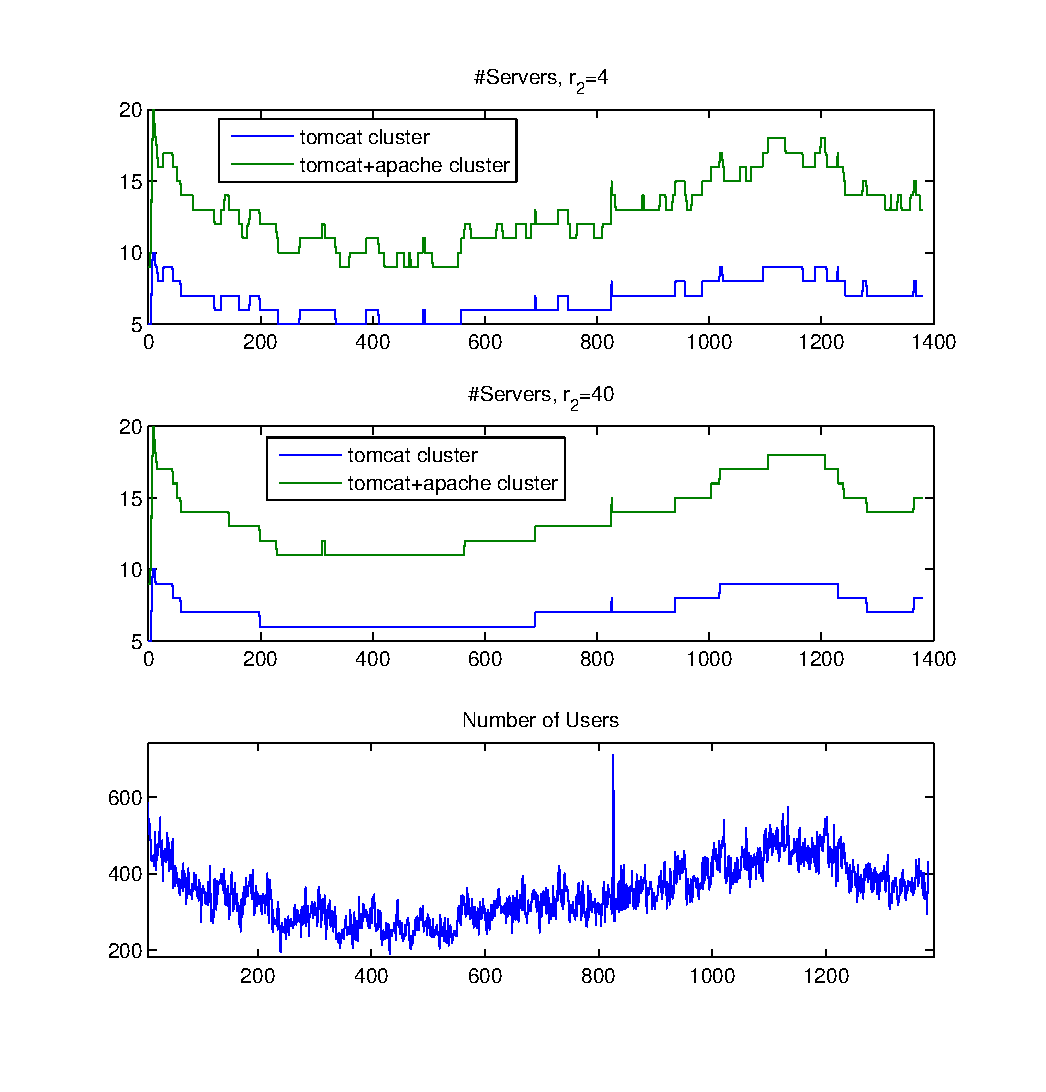
\includegraphics[width=18cm]{./image/autoscaling_different_trashing_cost.eps}
%
%\caption[Represents the placement decisions for a small service center using MPC.]
%{Reme step. }
%
%\label{fig:overal_optimal_example}  
%
%\end{center}
%
%\end{figure}
%


 \section{Work That Remains}  
  Examples should be added to show how the clusters are scaled automatically in response to changes in the disturbance inputs.   Disturbances include the workload component  and the SLA's.
 


